In a model based MP a stock assessment model is used to derive stock status relative to limit and target reference points and based on this to set a TAC. 

A limit requires something to be done before it is reached and a target is a reward for doing something good. The standard fisheries HCR is a hockey stick (\textbf{Figure} \ref{fig:hcr}) where for any biomass a corresponding fishing mortality is given, which is then used to derive a TAC. The hockey stick is defined by two points, the target fishing mortality ($F_{target}$) and a threshold ($B_{threshold}$)  that cause management action to be triggered if it is breached. Above $B_{threshold}$ $F_{target}$ defines a target level of fishing mortality that management seeks to achieve, below  $B_{threshold}$ F declines linearly to the limit biomass ($B_{lim}$).


\begin{figure*}[htbp]
\centering
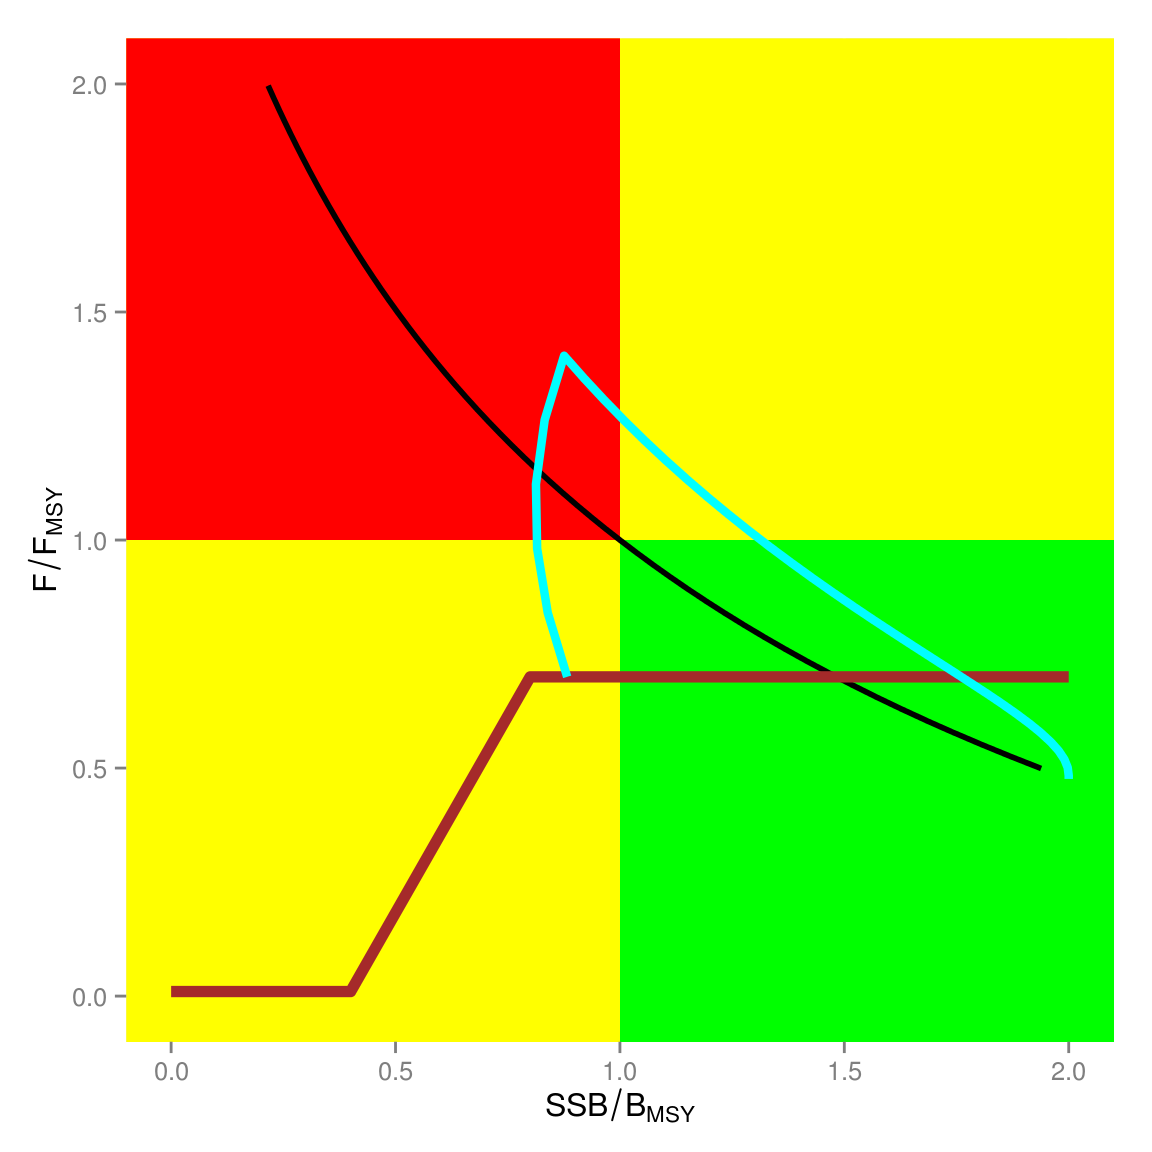
\includegraphics[width=6in]{../png/hcr.png}
\label{fig:hcr}
\caption{Harvest Control Rule (brown) plotted on a phase plot of harvest rate relative to $F_{MSY}$ and stock biomass relative to $B_{MSY}$;
the light line is the simulated stock and the black line is the replacement line.}
\end{figure*}


Setting targets and limits requires deciding upon the values used to define these two points. For example using a stock assessment there are severall potential reference points such as those based on maximum sustainable yield ($MSY$), i.e. the biomass at which this is achived ($B_{MSY}$ and the fishing mortlaity ($F_{MSY}$) that will achieve it.

The biomass of a stock next year ($B_{t+1}$) is equal to the biomass this year $B_{t}$, less the catch ($C_t$) plus the surplus production ($P_t$) i.e. 

\begin{equation}  B_{t+1}=B_{t}-C_{t}+P_{t}\end{equation}  

$P$ is given by the Pella-Tomlinson surplus production function \citep{pella1969generalized}

\begin{equation}\frac{r}{p}\cdot~B(1-(\frac{B}{K})^p)\end{equation}  

